\chapter{Teoretická část}
Some introductory text\dots







\section{Stávající metody}



\subsection{Rozpoznávání postav}
\subsection{Rozpoznávání částí těla}
\subsection{Rozpoznávání gest}
\begin{figure}[h]
\centering
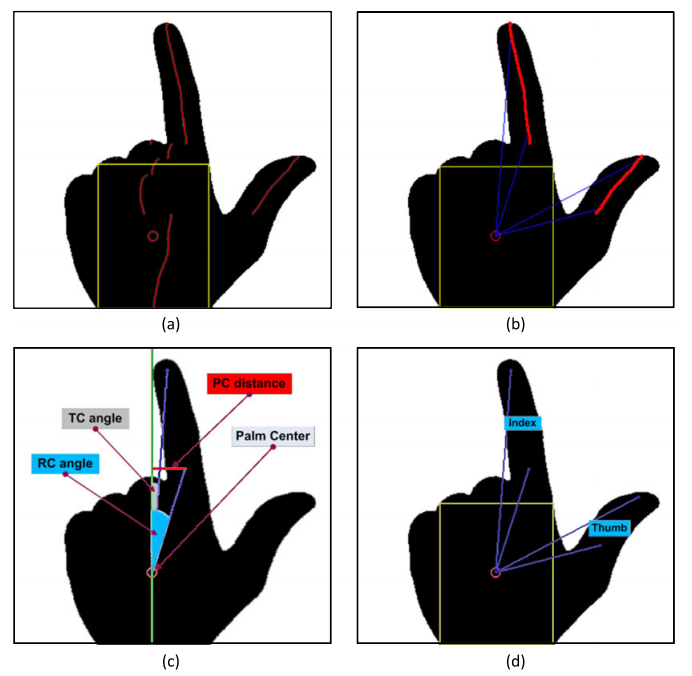
\includegraphics[width=0.9\linewidth]{fingers.png}
\caption{Vyobrazení definovaných pojmů, které lze využít k výpočtům pozic, na základě proporcionálních vlastností prstů. ~\cite{13} }
\end{figure}
\begin{center}
$RC_{angle} = 90 - tan^{-1} \frac{y_{r}-y_{pc}}{x_{r} - x_{pc}}$ \\
$TC_{angle} = 90 - tan^{-1} \frac{y_{ft}-y_{pc}}{x_{ft} - x_{pc}}$ 
\end{center}
\section{Aktuální aplikace} %využívajících rozpoznávání gest



\endinput
%%
%% End of file `ch01.tex'.
